\section{TPID Solver}

Our charged-puncture initial-data solver is based on existing
TwoPunctures-style methods. The discussion here follows closely the
presentation of Ref.~\cite{Bozzola2019}, as well as the original
TwoPunctures paper~\cite{Ansorg2004_TwoPunctures}. The solver is used to
construct initial data for two charged black holes separated along the
$x$ axis, with punctures located at $x=\pm b$. The user specifies the
bare parameters of the punctures, including their masses, charges, linear
momenta, and spins. These parameters determine the source terms that
enter the constraint equations.

The TPID solver uses a pseudo-spectral collocation method. In contrast
to a finite-difference method, where variables are stored on a grid and
derivatives are approximated using local stencils, a pseudo-spectral
method represents the unknown correction functions using global basis
functions. The equations are then enforced at a discrete set of
collocation points. Once the solution is obtained at these points, it is
interpolated onto the numerical grid used for the time evolution.

The coordinate system used by TwoPunctures is designed to cover all of
$\mathbb{R}^3$ with a single compactified computational domain. The
physical coordinates $(x,y,z)$ are parameterized by computational
coordinates $(A,B,\phi)$, where $A,B\in[-1,1]$ and
$\phi\in[0,2\pi]$. The transformation is given by
\begin{equation}
x
=
b
\frac{(1+A)^2+4}{(1+A)^2-4}
\frac{2B}{1+B^2},
\end{equation} 
\begin{equation}
y
=
b
\frac{4(1+A)}{4-(1+A)^2}
\frac{1-B^2}{1+B^2}
\cos\phi,
\end{equation}
\begin{equation}
z
=
b
\frac{4(1+A)}{4-(1+A)^2}
\frac{1-B^2}{1+B^2}
\sin\phi .
\end{equation}
These coordinates form a cylindrical-like coordinate system around the
$x$ axis, with the mapping depending on both $A$ and $B$. The punctures
are located on the $x$ axis, while the outer boundary of the compactified
domain corresponds to spatial infinity. In particular, the limit
$A\rightarrow 1$ maps to spatial infinity. This compactification makes it
straightforward to impose the boundary condition that the correction to
the conformal factor vanishes at infinity.

The computational coordinates are discretized using $n_A$, $n_B$, and
$n_\phi$ collocation points. An example of this grid is shown in
Fig.~\ref{fig:twopunctures_grid}. In the $A$ and $B$ directions, these
points are chosen from the roots of Chebyshev polynomials, which
concentrate resolution near the punctures and in regions where the
solution varies rapidly. The unknown correction functions are expanded
spectrally, and the expansion coefficients are determined by requiring
the constraint equations to be satisfied at the collocation points.

Because the constraint equations are nonlinear, the resulting algebraic
system is solved iteratively using a Newton--Raphson method. At each
iteration, the residuals of the constraint equations are evaluated at the
collocation points. These residuals measure the extent to which the
current approximate solution fails to satisfy the constraint equations.
For an exact solution, the residuals would vanish at every collocation
point. In practice, the Newton--Raphson iteration is continued until a
chosen norm of the residuals falls below a prescribed tolerance,
indicating that the constraints are satisfied to the desired numerical
accuracy. The resulting spectral solution is then interpolated from the
TwoPunctures collocation points onto the evolution grid used in the
numerical relativity simulation.

\begin{figure}[t]
    \centering
    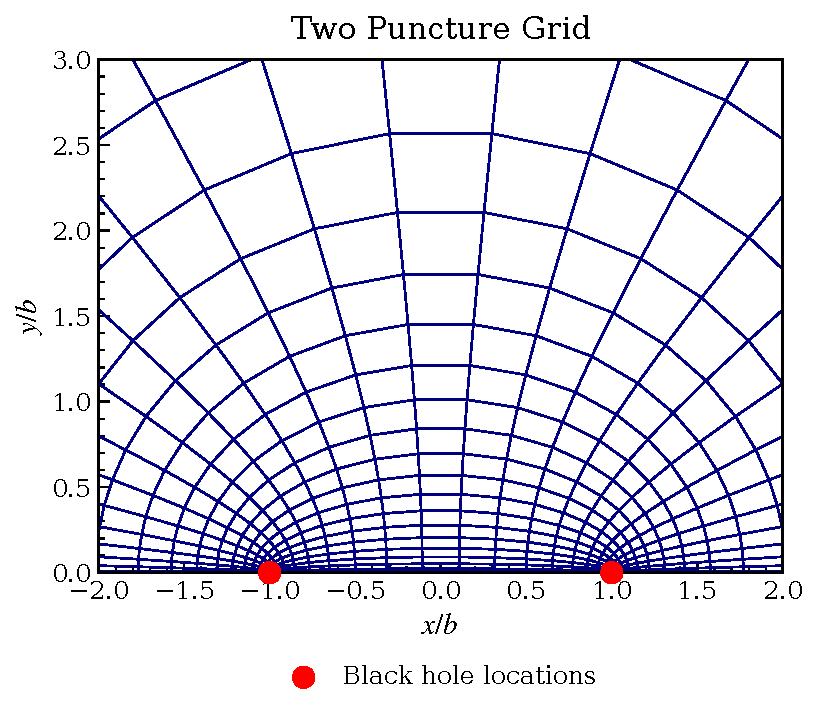
\includegraphics[width=0.75\textwidth]{Figures/twopunctures_grid.pdf}
    \caption{
    Example of the compactified TwoPunctures grid in a slice through the
    two punctures. The physical coordinates are shown in units of the
    half-separation $b$, with the black-hole punctures located at
    $x=\pm b$. The coordinate lines illustrate how the pseudo-spectral
    collocation points are distributed in the compactified domain before
    the resulting initial data are interpolated onto the evolution grid.
    The outer compactified boundary corresponds to spatial infinity and
    is outside the finite plotting window.
    }
    \label{fig:twopunctures_grid}
\end{figure}
